\documentclass[9pt,fleqn,twoside,twocolumn]{stdglobal}

\fancypagestyle{sectionstyle}{
  \fancyhf{}
  \fancyhead[L]{\footnotesize\itshape Seminar (Illustrative Visualization) 2021/2022}
  % \fancyfoot[C]{\footnotesize\bigskip\thepage/\pageref{LastPage}}
  % \fancyfoot{}
  \fancyfoot[C]{\footnotesize\bigskip\thepage}
  \fancyfoot[R]{\footnotesize\bigskip\copyright\ Markus Pawellek, \today}
  \renewcommand{\footrulewidth}{0.5pt}
  \renewcommand{\headrulewidth}{0pt}
}

\fancypagestyle{mainstyle}{
  \fancyhf{}
  \fancyfoot[C]{\footnotesize\bigskip\thepage}
  \fancyfoot[R]{\footnotesize\bigskip\copyright\ Markus Pawellek, \today}
  % \fancyhead[LO,RE]{\footnotesize \thetitle} %left
  % \fancyhead[RO,LE]{\footnotesize \theauthor} %right
  % \fancyhead[LO,RE]{\footnotesize \ \smallskip}
  \fancyhead[RO]{\footnotesize \@title \smallskip} %right
  \fancyhead[LE]{\footnotesize \@title \smallskip} %right
  \renewcommand{\headrulewidth}{0.5pt}
  \renewcommand{\footrulewidth}{0.5pt}
}

\usepackage{titlesec}
\titleformat{\section}{\normalfont\bfseries}{\thesection}{1em}{}

\title{%
  Photic Extremum Lines
}
%\subtitle{Seminar Report}
\author{Markus Pawellek}
\date{\today}

\hypersetup{
  pdftex,
  % pdfauthor={Your Name},
  % pdftitle={The Title},
  % pdfsubject={\@title},
  pdfkeywords={Non-Photorealistic Rendering; Feature Lines; View-Dependent Object-Space Algorithm; Contours; Silhouettes; Suggestive Contours; Photic Extremum Lines; Illumination; Interactive},
  % pdfproducer={Latex with hyperref},
  % pdfcreator={pdflatex, or other tool}
}

\bibliography{references}

\begin{document}

\selectlanguage{english}
\thispagestyle{sectionstyle}

\twocolumn[{\begin{@twocolumnfalse}%
  \begin{center}
    \Large
    \bfseries
    Photic Extremum Lines
  \end{center}%
  %\hfill\rule{0.5\textwidth}{0.5pt}\hfill
  \vspace{1pt}
  \begin{center}
    Markus Pawellek \\
    markus.pawellek@mailbox.org
  \end{center}
  \vspace{1em}
  \begin{center}
    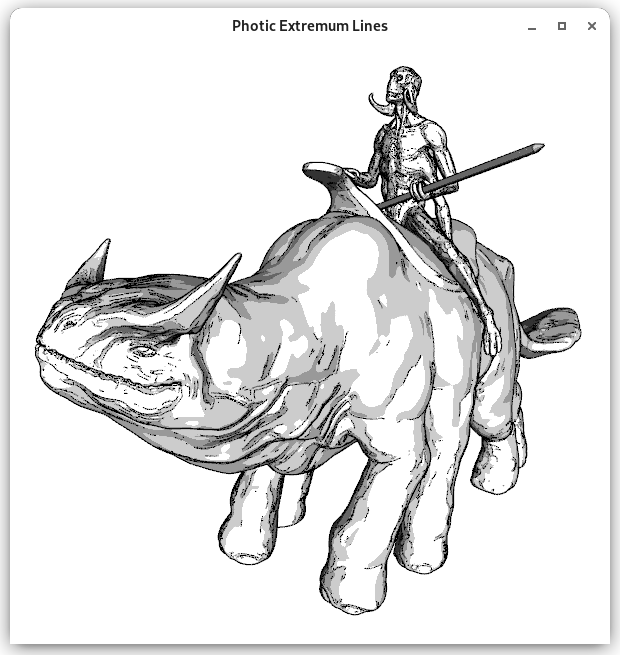
\includegraphics[width=0.24\textwidth,trim={15px 15 15 50},clip]{images/rider.png}
    \hfill
    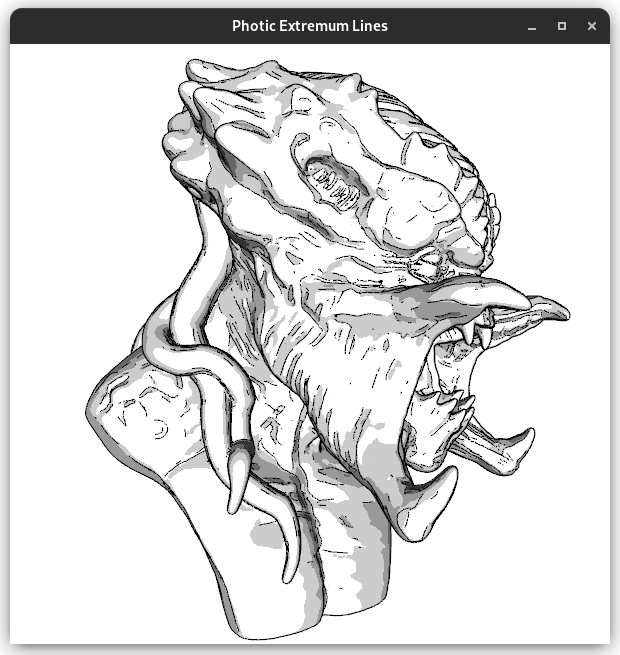
\includegraphics[width=0.24\textwidth,trim={15px 15 15 50},clip]{images/predator-intro.png}
    \hfill
    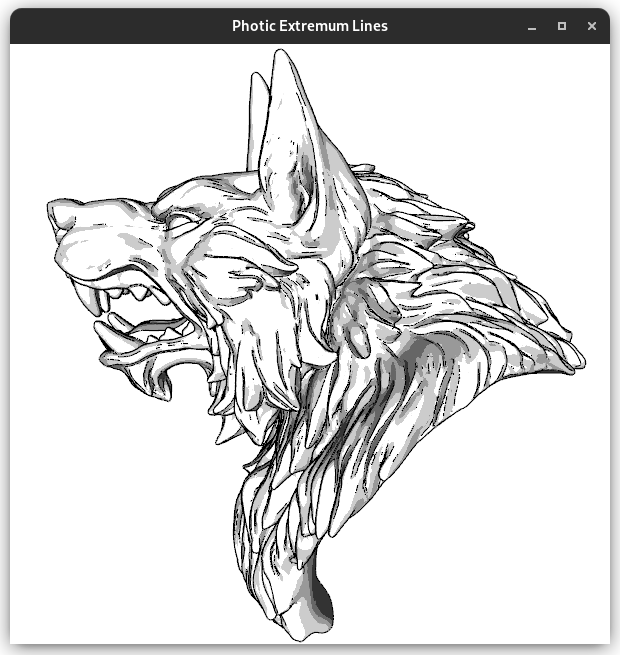
\includegraphics[width=0.24\textwidth,trim={15px 15 15 50},clip]{images/werewolf-intro.png}
    \hfill
    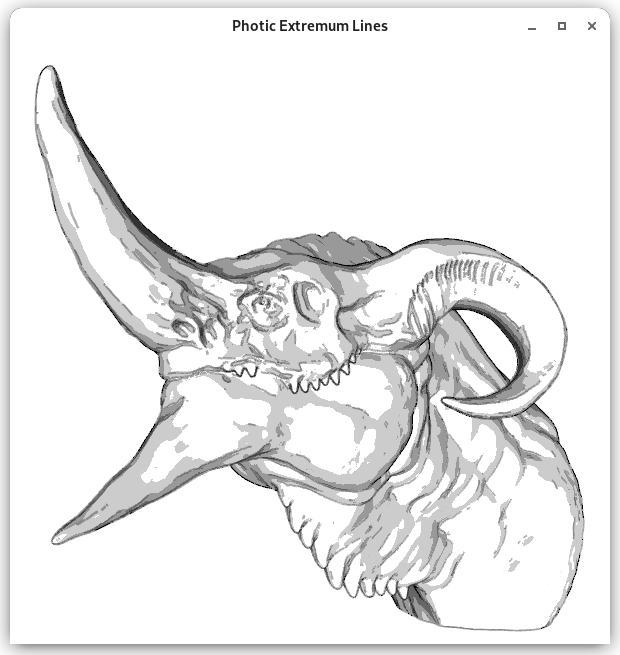
\includegraphics[width=0.24\textwidth,trim={15px 15 15 50},clip]{images/dragon-head-contour-pel-toon-shader.png}
  \end{center}
  \vspace{2em}
  \hrule
  \begin{abstract}
    \itshape
    \noindent
    Lorem ipsum dolor sit amet, consectetur adipisicing elit, sed do eiusmod
    tempor incididunt ut labore et dolore magna aliqua. Ut enim ad minim veniam,
    quis nostrud exercitation ullamco laboris nisi ut aliquip ex ea commodo
    consequat. Duis aute irure dolor in reprehenderit in voluptate velit esse
    cillum dolore eu fugiat nulla pariatur. Excepteur sint occaecat cupidatat non
    proident, sunt in culpa qui officia deserunt mollit anim id est laborum.
    \\

    \noindent
    \textbf{Keywords:}
    \parbox[t]{0.8\textwidth}{Non-Photorealistic Rendering, Feature Lines, View-Dependent Object-Space Algorithm, Contours, Silhouettes, Suggestive Contours, Photic Extremum Lines, Illumination, Interactive}
  \end{abstract}
  \hrule
  \vspace{3em}
\end{@twocolumnfalse}}]

\begin{figure*}
    \centering
    \begin{subfigure}[b]{0.24\textwidth}
      \centering
      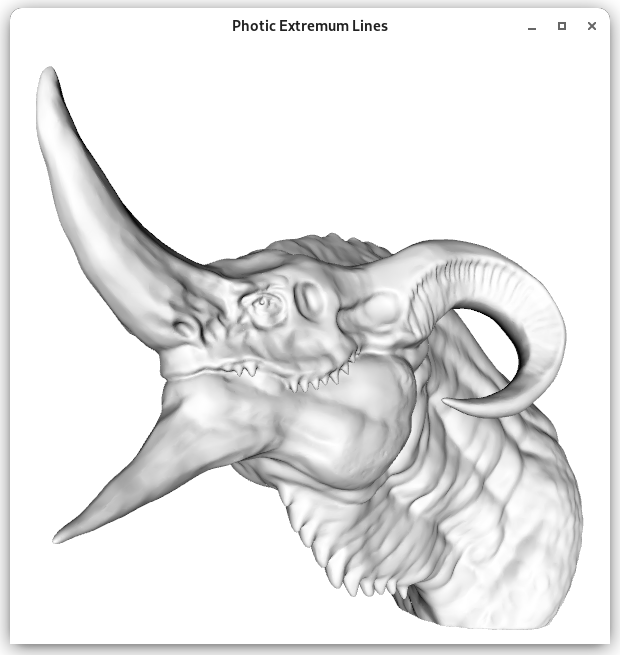
\includegraphics[width=0.95\textwidth,trim={15px 15 15 50},clip]{images/dragon-head-vertex-lighting.png}
      \caption{Illumination}
    \end{subfigure}%
    \hfill%
    \begin{subfigure}[b]{0.24\textwidth}
      \centering
      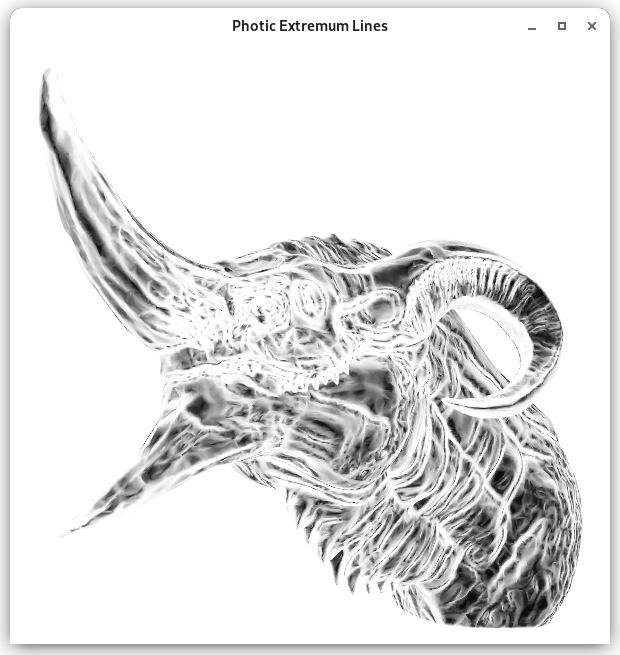
\includegraphics[width=0.95\textwidth,trim={15px 15 15 50},clip]{images/dragon-head-light-variation.png}
      \caption{Variation}
    \end{subfigure}%
    \hfill%
    \begin{subfigure}[b]{0.24\textwidth}
      \centering
      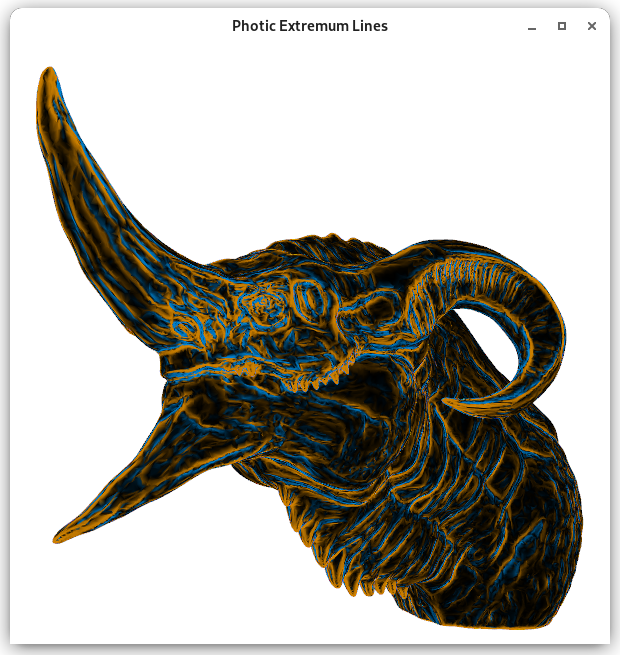
\includegraphics[width=0.95\textwidth,trim={15px 15 15 50},clip]{images/dragon-head-light-variation-slope.png}
      \caption{Variation Slope}
    \end{subfigure}%
    \hfill
    \begin{subfigure}[b]{0.24\textwidth}
      \centering
      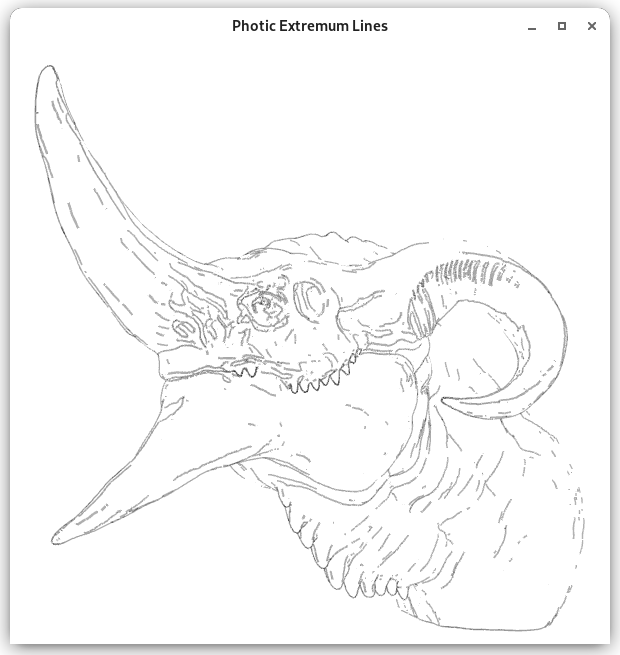
\includegraphics[width=0.95\textwidth,trim={15px 15 15 50},clip]{images/dragon-head-pel-shader.png}
      \caption{PELs}
    \end{subfigure}%
    \caption{\textbf{Short Summary Part}\\
    Lorem ipsum dolor sit amet, consectetur adipisicing elit, sed do eiusmod
    tempor incididunt ut labore et dolore magna aliqua. Ut enim ad minim veniam,
    quis nostrud exercitation ullamco laboris nisi ut aliquip ex ea commodo
    consequat. Duis aute irure dolor in reprehenderit in voluptate velit esse
    cillum dolore eu fugiat nulla pariatur. Excepteur sint occaecat cupidatat non
    proident, sunt in culpa qui officia deserunt mollit anim id est laborum.}
  \end{figure*}

\section{Introduction}
  Lorem ipsum dolor sit amet, consectetur adipisicing elit, sed do eiusmod
  tempor incididunt ut labore et dolore magna aliqua. Ut enim ad minim veniam,
  quis nostrud exercitation ullamco laboris nisi ut aliquip ex ea commodo
  consequat. Duis aute irure dolor in reprehenderit in voluptate velit esse
  cillum dolore eu fugiat nulla pariatur. Excepteur sint occaecat cupidatat non
  proident, sunt in culpa qui officia deserunt mollit anim id est laborum.

\section{Related Work}

\section{Mathematical Preliminaries}
  \begin{figure}
    \centering
    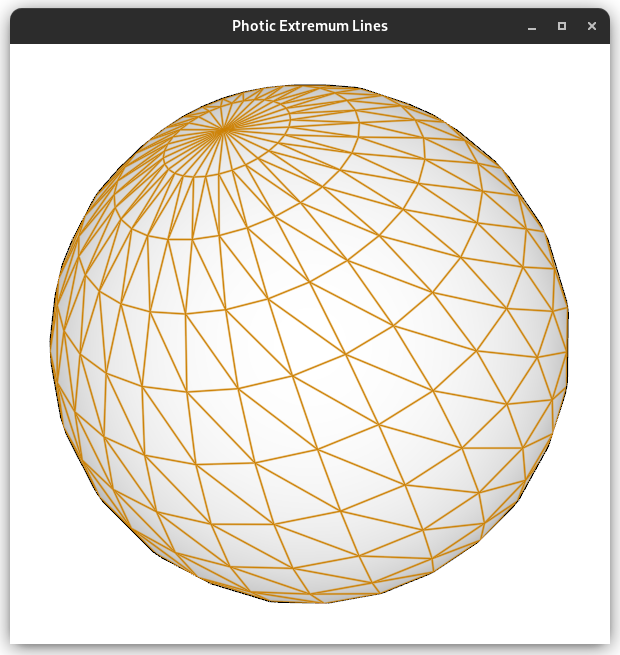
\includegraphics[width=0.6\linewidth,trim={15px 15 15 50},clip]{images/sphere-wireframe.png}
    \caption{Triangulated Meshes}
  \end{figure}

\section{Photic Extremum Lines}

\section{Algorithm}

  \begin{figure}
    \centering
    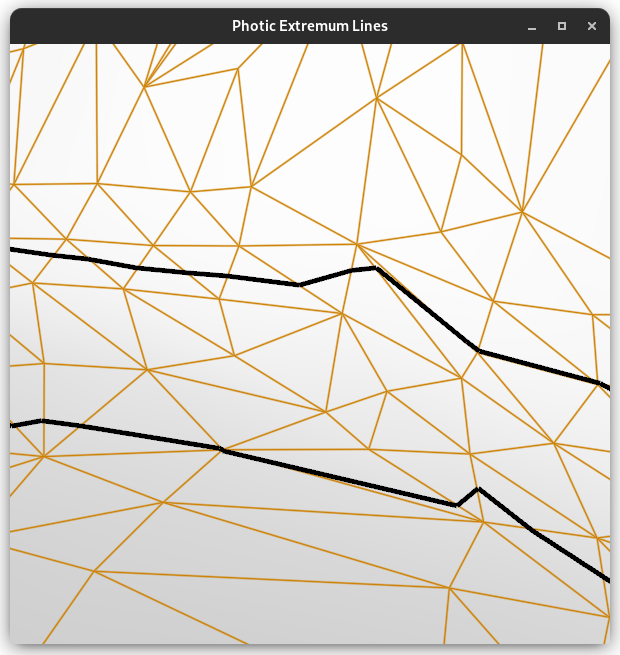
\includegraphics[width=\linewidth,trim={15px 15 15 50},clip]{images/subpolygon-lines.png}
    \caption{Sub-Polygon Feature Lines}
  \end{figure}

\section{Implementation}

\section{Results and Comparison}

  \begin{figure*}
      \centering
      \begin{subfigure}[b]{0.24\textwidth}
        \centering
        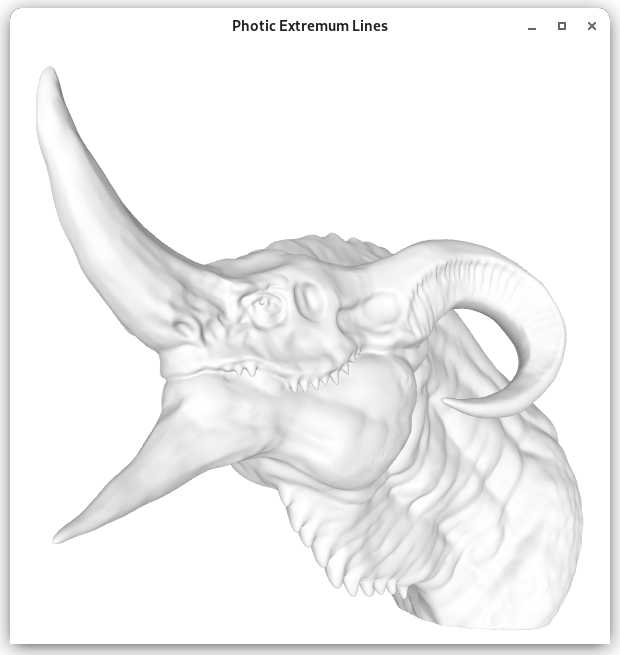
\includegraphics[width=0.95\textwidth,trim={15px 15 15 50},clip]{images/dragon-head-viewer-shader.png}
        \caption{Illumination}
      \end{subfigure}%
      \hfill%
      \begin{subfigure}[b]{0.24\textwidth}
        \centering
        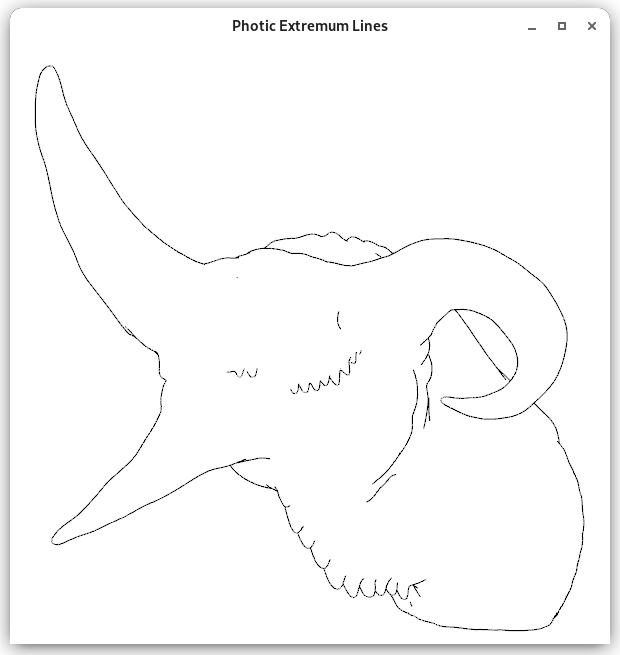
\includegraphics[width=0.95\textwidth,trim={15px 15 15 50},clip]{images/dragon-head-contours.png}
        \caption{Contours}
      \end{subfigure}%
      \hfill%
      \begin{subfigure}[b]{0.24\textwidth}
        \centering
        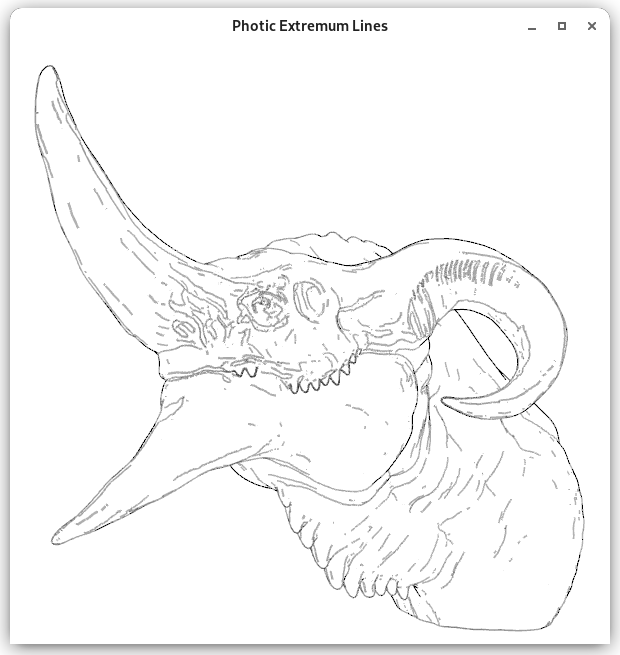
\includegraphics[width=0.95\textwidth,trim={15px 15 15 50},clip]{images/dragon-head-contour-pel-shader.png}
        \caption{Contours and PELs}
      \end{subfigure}%
      \hfill
      \begin{subfigure}[b]{0.24\textwidth}
        \centering
        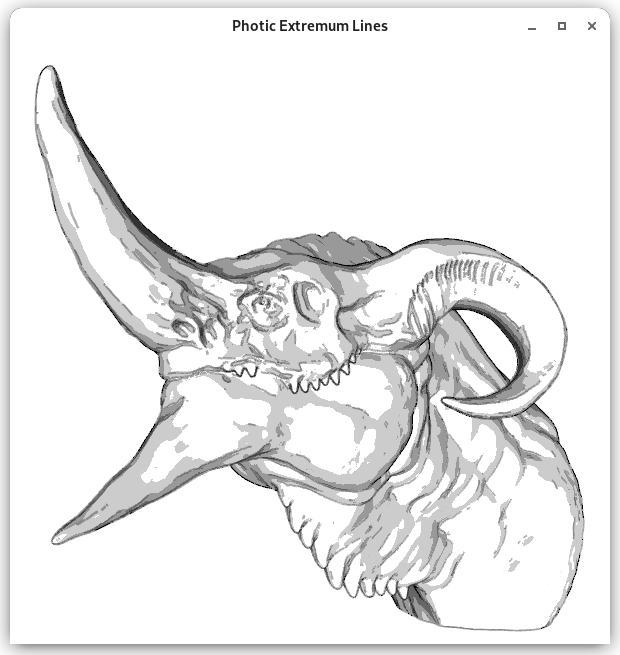
\includegraphics[width=0.95\textwidth,trim={15px 15 15 50},clip]{images/dragon-head-contour-pel-toon-shader.png}
        \caption{Contours, PELs, and Toon}
      \end{subfigure}%
      \caption{\textbf{Short Summary Part}\\
      Lorem ipsum dolor sit amet, consectetur adipisicing elit, sed do eiusmod
      tempor incididunt ut labore et dolore magna aliqua. Ut enim ad minim veniam,
      quis nostrud exercitation ullamco laboris nisi ut aliquip ex ea commodo
      consequat. Duis aute irure dolor in reprehenderit in voluptate velit esse
      cillum dolore eu fugiat nulla pariatur. Excepteur sint occaecat cupidatat non
      proident, sunt in culpa qui officia deserunt mollit anim id est laborum.}
    \end{figure*}

  \begin{figure}
    \centering
    \begin{subfigure}[b]{0.49\linewidth}
      \centering
      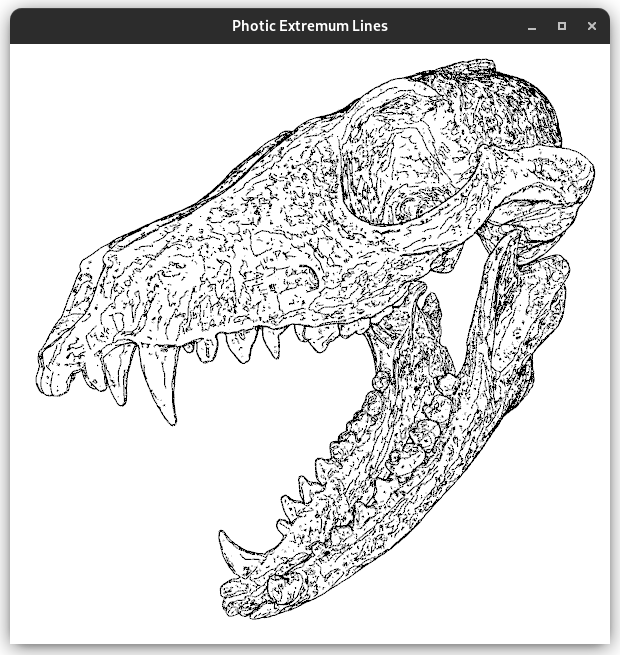
\includegraphics[width=\textwidth,trim={15px 15 15 50},clip]{images/fox-skull-threshold-low.png}
      \caption{Low}
    \end{subfigure}
    \begin{subfigure}[b]{0.49\linewidth}
      \centering
      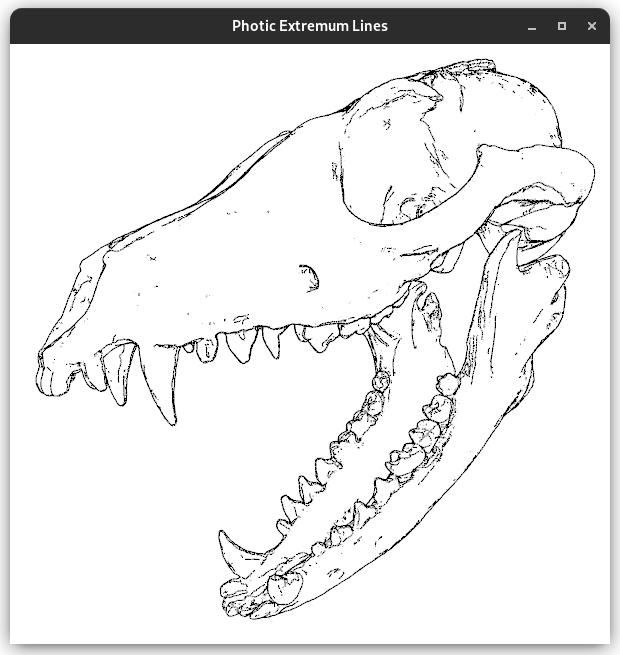
\includegraphics[width=\textwidth,trim={15px 15 15 50},clip]{images/fox-skull-threshold-mid.png}
      \caption{Mid}
    \end{subfigure}
    \caption{Effect of thresholding}
  \end{figure}

  \begin{figure}
    \centering
    \begin{subfigure}[b]{0.49\linewidth}
      \centering
      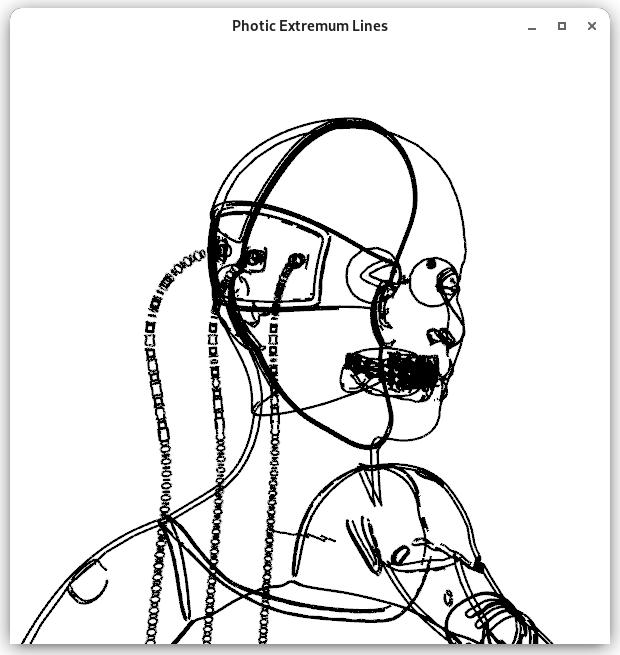
\includegraphics[width=\textwidth,trim={15px 15 15 50},clip]{images/cyborg-contour-pel-hidden-shader.png}
      \caption{Off}
    \end{subfigure}
    \begin{subfigure}[b]{0.49\linewidth}
      \centering
      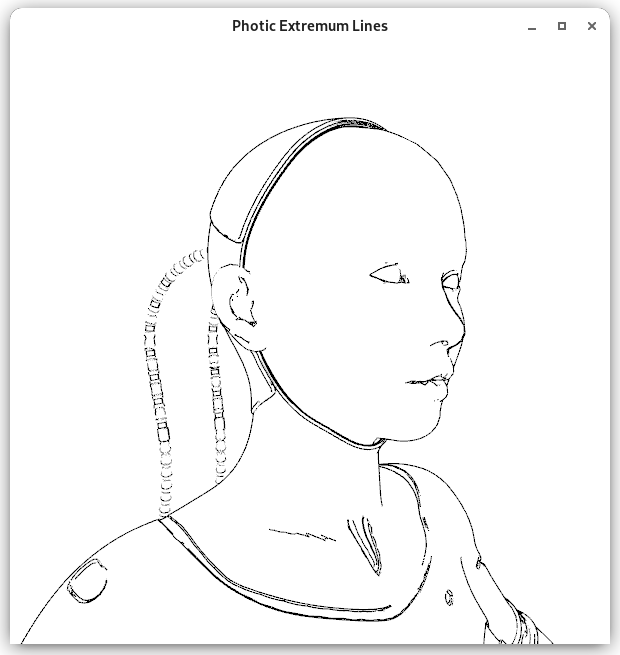
\includegraphics[width=\textwidth,trim={15px 15 15 50},clip]{images/cyborg-contour-pel-shader.png}
      \caption{On}
    \end{subfigure}
    \caption{Two-Pass Rendering for Hidden Line Removal}
  \end{figure}

  \begin{figure}
    \centering
    \begin{subfigure}[b]{\linewidth}
      \centering
      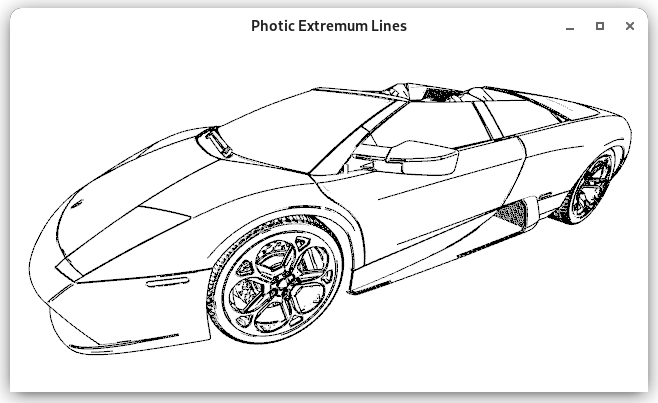
\includegraphics[width=\textwidth,trim={15px 15 15 50},clip]{images/lamborghini-front.png}
      \caption{Front}
    \end{subfigure}
    \begin{subfigure}[b]{\linewidth}
      \centering
      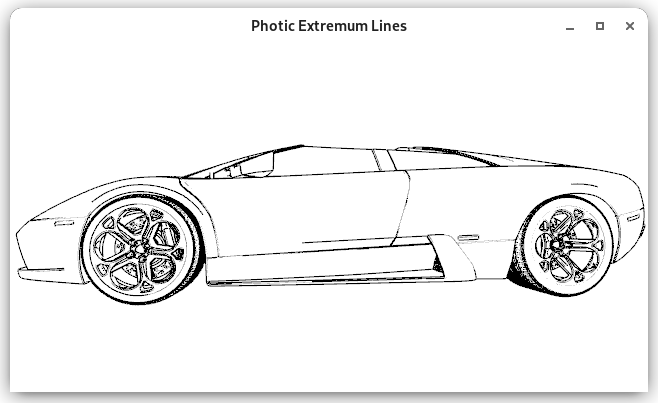
\includegraphics[width=\textwidth,trim={15px 15 15 50},clip]{images/lamborghini-side.png}
      \caption{Side}
    \end{subfigure}
    \caption{Nearly Perfect Line Extraction for Smooth Objects}
  \end{figure}

  \begin{figure}
    \centering
    \begin{subfigure}[b]{0.49\linewidth}
      \centering
      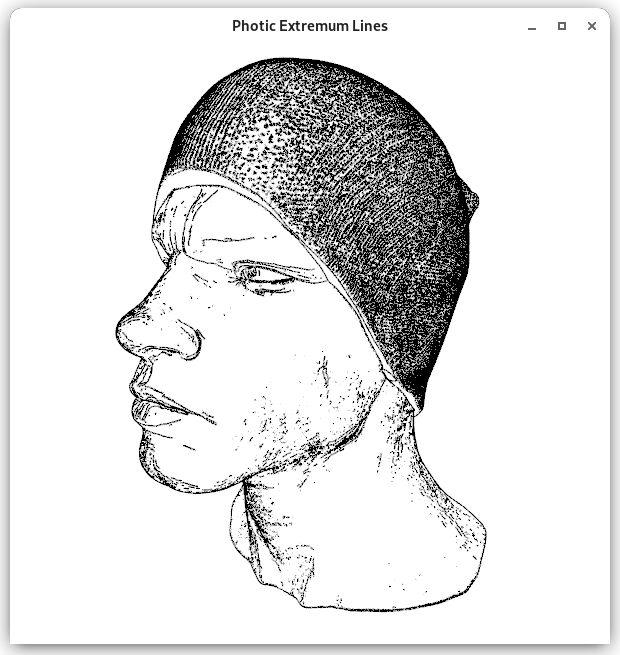
\includegraphics[width=\textwidth,trim={15px 15 15 50},clip]{images/head-contour-pel-shader.png}
      \caption{Contours and PELs}
    \end{subfigure}
    \begin{subfigure}[b]{0.49\linewidth}
      \centering
      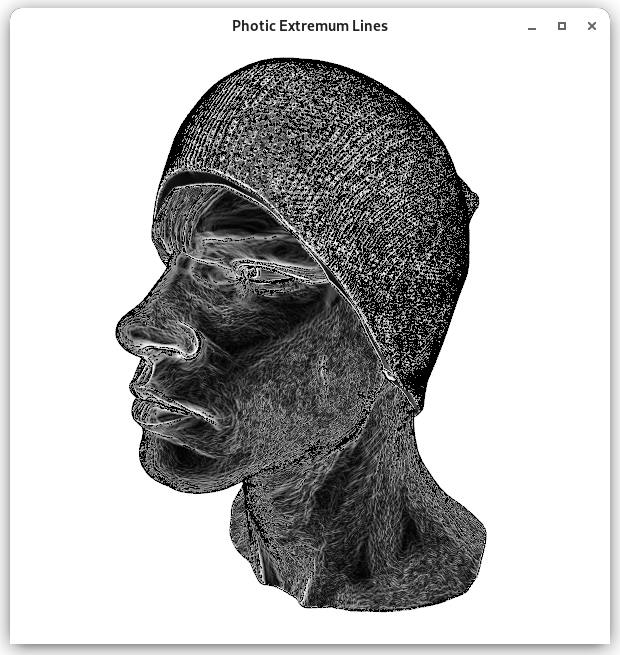
\includegraphics[width=\textwidth,trim={15px 15 15 50},clip]{images/head-light-variation.png}
      \caption{Variation}
    \end{subfigure}
    \caption{Erroneous Line Extraction for Noisy Objects}
  \end{figure}

\section{Conclusions}

\nocite{*}
\AtNextBibliography{\footnotesize}
\printbibliography[heading=bibintoc]

\appendix

\end{document}
